\documentclass[12pt,letterpaper]{article}
\usepackage[secthm,mdthm,simplethm]{beel}
\usepackage[utf8]{inputenc}
\usepackage{graphicx, tcolorbox}
\usepackage[margin = 1in, top = 0.8in,bottom = 0.8in]{geometry}
\usepackage{amsmath,amsfonts,amsthm,amssymb}
\usepackage{array,comment,enumitem}
\usepackage{mathtools,thmtools}
\usepackage{multicol,tabto,setspace}
\usepackage{tikz,pgfplots,tikz-cd,venndiagram,forest}
\usepackage[all]{xy}
\usepackage{listings,fancyhdr}
\usepackage{tikz,tikz-3dplot} 
\pagestyle{fancy}

\headheight = 15 pt
\lhead{Bill Li}
\rhead{Groups, Rings, and Fields}
\cfoot{\thepage}
\pgfplotsset{compat = 1.15}
\usetikzlibrary{fadings}
\parindent = 0 in
\hbadness = 10000
\tolerance = 10000

\renewcommand{\qedsymbol}{$\blacksquare$}
\renewcommand{\bar}{\overline}
\renewcommand{\b}{\mathbb}
\renewcommand{\c}{\mathcal}
\newcommand{\s}{\mathscr}

\begin{document}

\thispagestyle{empty}
$ $
\vfill
\begin{center}

\centerline{\huge \textbf{Math 250, Fall 2019}}
\centerline{\Large \textbf{Groups, Rings and Fields, Fall 2019}} 
\centerline{Richard E. Borcherds, 219 Dwinelle, 9:30-11AM}
\end{center}
\vfill
$ $
\newpage
\thispagestyle{empty}
\tableofcontents
\newpage
\setcounter{page}{1}
%!TEX root = ./main.tex
\section{Groups}
There are two definitions to define a group.
\begin{definition}[Concrete definition]
	A group is a symmetries of something 1:1 map preserving ``structure''.
\end{definition}
\begin{example}
	Consider the rotation of a rectangle, we have a group of order $4$.
\end{example}
\begin{example}
	Consider the rotation of a icosahedron, we are able to obtain a group of order $60$.
	\tdplotsetmaincoords{60}{100}
	\begin{center}
	    \begin{tikzpicture}
	    	[tdplot_main_coords,scale=1,line join=round]
	    \pgfmathsetmacro\a{2}
	    \pgfmathsetmacro{\phi}{\a*(1+sqrt(5))/2}
	    \path 
	    coordinate(A) at (0,\phi,\a)
	    coordinate(B) at (0,\phi,-\a)
	    coordinate(C) at (0,-\phi,\a)
	    coordinate(D) at (0,-\phi,-\a)
	    coordinate(E) at (\a,0,\phi)
	    coordinate(F) at (\a,0,-\phi)
	    coordinate(G) at (-\a,0,\phi)
	    coordinate(H) at (-\a,0,-\phi)
	    coordinate(I) at (\phi,\a,0)
	    coordinate(J) at (\phi,-\a,0)
	    coordinate(K) at (-\phi,\a,0)
	    coordinate(L) at (-\phi,-\a,0); 
	    \draw[dashed, thick]    (B) -- (H) -- (F) 
	    (D) -- (L) -- (H) --cycle 
	    (K) -- (L) -- (H) --cycle
	    (K) -- (L) -- (G) --cycle
	    (C) -- (L) (B)--(K) (A)--(K)
	    ;

	        \draw[ultra thick]
	        (A) -- (I) -- (B) --cycle 
	        (F) -- (I) -- (B) --cycle 
	        (F) -- (I) -- (J) --cycle
	        (F) -- (D) -- (J) --cycle
	        (C) -- (D) -- (J) --cycle
	        (C) -- (E) -- (J) --cycle
	        (I) -- (E) -- (J) --cycle
	        (I) -- (E) -- (A) --cycle
	        (G) -- (E) -- (A) --cycle
	        (G) -- (E) -- (C) --cycle
	        ; 
			 %\foreach \point/\position in {A/right,B/below,C/above,D/left,E/{above right},F/below,G/above,H/left,I/below,J/right,K/below,L/left}
			%{
			    %\fill (\point) circle (1.5pt);
			    %\node[\position=3pt] at (\point) {$\point$};
			%}

\end{tikzpicture} \\
Image of a Icosahedron
\end{center}
\end{example}
\begin{example}
	Let $V$ be a $n$-dimensional over $\b R$. The general linear group $GL_n(\b R)$, all matrices with $\det \neq 0$ from a group. 
\end{example}
\begin{definition}[Abstract Definition, Cayley]
	A group is a set $G$ with a binary operation $a + b$ or $a \times b$ or $a \circ b$ or $ab$ (notation sucks) such that
	\begin{enumerate}
		\item Identity element $0$, $1$, or $e$, i,e $a1 = 1a = a$.
		\item Each element has inverse $a^{-1}$, i,e $aa^{-1} = a^{-1}a = 1$.
		\item Associative $(ab)c = a(bc)$ for all $a,b,c \in G$
	\end{enumerate}
\end{definition}
\begin{definition}
	A group $G$ acts on $S$ means given operation 
	\[ G \times S \to S \]
	such that $1s = s$ and $a(bs) = ab(s)$.
\end{definition}
\begin{example}
	Let $G$ be the icosahedron group and let $S$ be the icosahedron.
\end{example}

\begin{question}
	How does $G$ acts on $G$?
\end{question}
\begin{definition}
	There are 8 different types of actions
	\begin{enumerate}
		\item $g(s) = s$, left action (trivial)
		\item $g(s) = gs$
		\item $g(s) = sg^{-1}$
		\item $g(s) = gsg^{-1}$, adjoint action
	\end{enumerate}
	Note that all of these are left actions of the group, then similarly there are also 4 right group actions. $S \times G \to S$
	\begin{enumerate}
		\item $sg = s$
		\item $sg = sg$
		\item $sg = g^{-1} s$
		\item $sg = g^{-1}sg$
	\end{enumerate}
\end{definition}
\begin{remark}
	$g(s) = gs, g(s) = sg^{-1}, sg = sg, sg = g^{-1}s$ does not preserve group operation of $S$.
\end{remark}
We let $G$ act on $S(=G)$ by $g(s) = gs$. This means $G$ into subset of all permutations of $S(=G)$. Now we want to add extra ``structure'' to $S$ so $G$ is exactly symmetries of $S$ with this structure.

Extra structure is \textbf{right} action of $G$ on $S$. We now have 3 copies of $G$
\begin{enumerate}
	\item Set $S(=G)$.
	\item $G$ acting on \textbf{right} on $S$ $\leftarrow$ part of structure
	\item $G$ acting on \textbf{left} on $S$ $\leftarrow$ symmetry group
\end{enumerate}
\begin{example}[Cayley Graph of 4 elements]
	$ $
	\begin{center}
		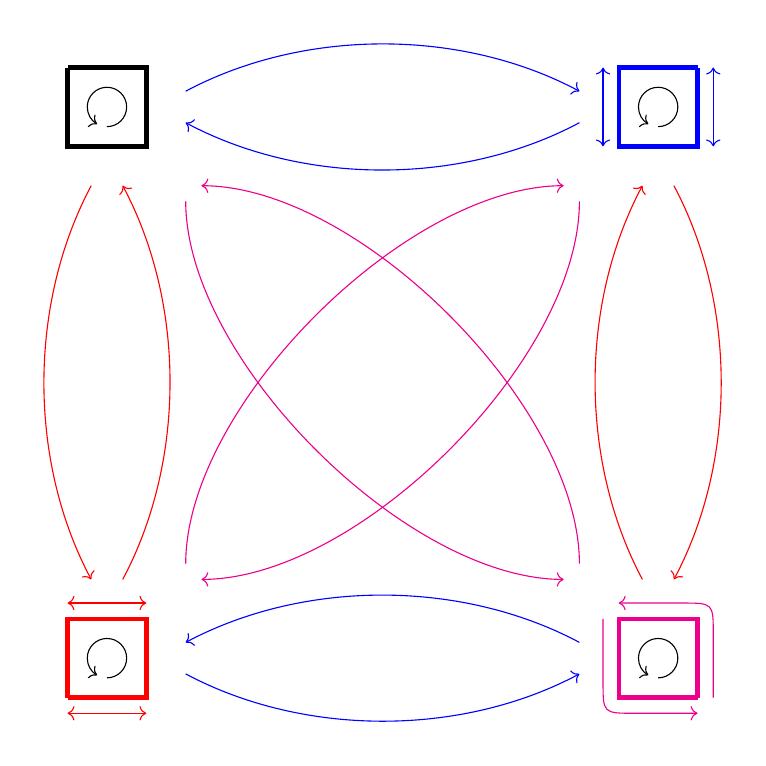
\begin{tikzpicture}
		\draw[color = blue, ultra thick] (4,4)--(4,3)--(3,3)--(3,4)--(4,4);
		\draw[color = red, ultra thick] (-4,-4)--(-4,-3)--(-3,-3)--(-3,-4)--(-4,-4);
		\draw[color = magenta, ultra thick] (4,-4)--(4,-3)--(3,-3)--(3,-4)--(4,-4);
		\draw[ultra thick] (-4,4)--(-4,3)--(-3,3)--(-3,4)--(-4,4);
		\draw[->] (3.5,3.25) arc (270:600:0.25);
		\draw[->] (-3.5,3.25) arc (270:600:0.25);
		\draw[->] (3.5,-3.75) arc (270:600:0.25);
		\draw[->] (-3.5,-3.75) arc (270:600:0.25);
		\draw[<->, color = blue] (4.2,3) -- (4.2,4);
		\draw[<->, color = blue] (2.8,3) -- (2.8,4);
		\draw[<->, color = red] (-4,-2.8) -- (-3,-2.8);
		\draw[<->, color = red] (-4,-4.2) -- (-3,-4.2);
		\draw[->, color = magenta] (2.8,-3) -- (2.8,-3.8) .. controls (2.8,-4.2) .. (3.2,-4.2) -- (4,-4.2);
		\draw[->, color = magenta] (4.2,-4) -- (4.2,-3.2) .. controls (4.2,-2.8) .. (3.8,-2.8) -- (3,-2.8);
		\draw[->, color = magenta] (2.5,2.3) .. controls +(down:20mm) and +(right:20mm) .. (-2.3,-2.5);
		\draw[->, color = magenta] (-2.5,-2.3) .. controls +(up:20mm) and +(left:20mm) .. (2.3,2.5);
		\draw[->, color = magenta] (2.5,-2.3) .. controls +(up:20mm) and +(right:20mm) .. (-2.3,2.5);
		\draw[->, color = magenta] (-2.5,2.3) .. controls +(down:20mm) and +(left:20mm) .. (2.3,-2.5);
		\draw[->, color = blue] (2.5,3.3) .. controls (1,2.5) and (-1,2.5) .. (-2.5,3.3);	
		\draw[<-, color = blue] (2.5,3.7) .. controls (1,4.5) and (-1,4.5) .. (-2.5,3.7);	
		\draw[->, color = blue] (2.5,-3.3) .. controls (1,-2.5) and (-1,-2.5) .. (-2.5,-3.3);	
		\draw[<-, color = blue] (2.5,-3.7) .. controls (1,-4.5) and (-1,-4.5) .. (-2.5,-3.7);
		\draw[->, color = red] (3.7,2.5) .. controls (4.5,1) and (4.5,-1) .. (3.7,-2.5);
		\draw[<-, color = red] (3.3,2.5) .. controls (2.5,1) and (2.5,-1) .. (3.3,-2.5);
		\draw[->, color = red] (-3.7,2.5) .. controls (-4.5,1) and (-4.5,-1) .. (-3.7,-2.5);
		\draw[<-, color = red] (-3.3,2.5) .. controls (-2.5,1) and (-2.5,-1) .. (-3.3,-2.5);
		\end{tikzpicture}
	\end{center}
	We get colored (directed) graph arrow gives \textbf{right} action of $G$, which is not the same as the \textbf{left} action.
\end{example}
\begin{remark}
	Goals of group theory
	\begin{enumerate}
		\item Classify all groups
		\item Given a group $G$, find all ways $G$ acts on something.
	\end{enumerate}
\end{remark}
\begin{example}
	Linear representation = actions of $G$ over vector space.

	Permutation = actions of $G$ over on a set.
\end{example}
\begin{definition}
	A homomorphism $f: G \to H$ map preserving group structure. i.e. $f(gh) = f(g)f(h)$.

	A isomorphism is a homomorphism that is a bijection. 

	The kernel of $f$ is the set of elements such that it maps to the trivial element of $H$ 
\end{definition}
\begin{example}
	Consider the function
	\[ \mathrm{exp} : \langle \b R, + \rangle \to \langle \b R^*, \cdot \rangle\]
	exp is a isomorphism from $\b R$ to $R_{> 0}$
\end{example}
\begin{example}
	Consider the function
	\[ \mathrm{exp} : \langle \b C, + \rangle \to \langle \b C^*, \cdot \rangle\]
	kernel = elements $2\pi i n, n \in \b Z$.
\end{example}
\begin{example}[Number Theory]
	Consider $\b Z/4 \b Z$ integers mod $4$. and $\left( \b Z/ 5 \b Z \right)^*$ nonzero integers mod $5$ under multiplication.
\end{example}
\begin{example}
	Consider the function :
	\[ \mathrm{det} : GL_n(\b R) = \b R^*\]
	is a homomorphism.

	kernel = $SL_n(\b R)$ = special linear group.
\end{example}
\begin{theorem}[Lagrange's Theorem]
	If $H$ is a subgroup of $G$, order of $H$ divides order of $G$. ($G$ is finite)
\end{theorem}
\begin{lemma}
	2 cosets either are the same or disjoint.
\end{lemma}
\begin{proof}
    If $aH \cap bH = \varnothing$, then the proof is done. \\
    Now we suppose $aH \cap bH \neq \varnothing$, then we know that $ah_1 = bh_2$ for some element in $aH$ and $bH$. We compute $ah_1 = bh_2 \implies h_1 = a^{-1}bh_2 \implies a^{-1}b = h_1h_2^{-1} \implies a^{-1}b \in H$. Then we know that $aH = bH$. \\
    We can use a similar argument to show that this works for the right cosets as well. This is left as an exercises to the reader. 
\end{proof}
\begin{lemma}
	Any cosets have the same size.
\end{lemma}
\begin{proof}
    We can simply prove that $\phi: h \mapsto bh$ is bijective, therefore $|H| = |bH|$. \\
    This proof is trivial and is left as an exercise to the reader. (Hint: prove that $\phi$ is injective and say it's surjective by construction)
\end{proof}
\begin{proof}
	Suppose $G$ acts on $S$. Pick $s \in S$, put $H = $set of elements fixing $s$ such that $hs = s$, then $H$ is a subgroup of $G$.

	Given a subgroup $H$ of $G$, we can find set $S$ acted on by $G$, $s \in S$. $H$ = things fixed in $S$.

	Given $g,h (H \subseteq G)$. $S = $ left cosets of $H$. 

	we get action of $G$ on set of cosets by putting $g(aH) = (ga)H$. (well-defined left as an exercise)

	Therefore $|G| = |H| \times $ number of cosets. Therefore the order of $H$ divides the order of $H$.
\end{proof}
\begin{theorem}
	If $g \in G$, then the order of $g$ divides divides order of $G$.
\end{theorem}
\begin{corollary}
	If $G$ is prime order, it is cyclic
\end{corollary}
\begin{proof}
	Pick any element $g \neq 1$. Order divided $p$, so $p$ is primes. so $G = $ powers of $g$
\end{proof}
\begin{example}
	List of all groups
	\begin{enumerate}
		\item Order 1 : Trivial group
		\item Order 2 : 1 group $\b Z/2\b Z$, $0,1$.
		\item Order prime $p$ : Integer $\mod p$.
		\item Order 4 : Cyclic group $\b Z/4 \b Z$ and symmetry of a rectangle. These are not isomorphic as the symmetry group of rectangle does not have a element of order $4$. 

		\item Classify all groups with $g^2 = 1$ for all $g$. We want to show that group is abelian, or $gh = hg$ for all $g,h \in G$. This follows because $ghgh = (gh)^2 = 1 = h^2g^2 = hhgg \implies hg = gh$.		 Since $G$ is abelian, we can write group operation as $+$. Notice that $G$ is a vector space over field of order $2$, namely $\b Z/2 \b Z$. so $h$ has a basis, and is isomorphic to $\left( \b Z/2\b Z\right)^n$($n$-dimensional vector space) to some $n$. So there is only $1$ other group of order $4$.
	\end{enumerate}
\end{example}
\begin{definition}
	Suppose $G,H$ are groups, then the product(sum) of the group is defined as follows
	\[ G \times H = \text{set of pairs} (g,h) \]
	and the operation is defined as 
	\[ (g_1,h_1)(g_2,h_2) = (g_1g_2,h_1h_2)\]
\end{definition}
\begin{example}
	symmetry of rectangle is isomorphic to $\b Z/2 \b Z \times \b Z/2 \b Z$.
\end{example}
\begin{example}
	$\b C^* = S \times \b R_{>0}$, where $S$ is the circle group. Notice that this is the polar decomposition of complex numbers.
\end{example}
\begin{definition}
	The product(sum) of groups are elements $(g_1, g_2, \ldots)$ such that all but finite number of $g_i$ are trivial.
\end{definition}
\begin{example}
	$\b Q^* = $ infinite sum of groups $\b Z/2 \b Z + \b Z /3 \b Z + \b Z /5 \b Z + \ldots$. This follows by fundamental theorem of arithmetic.
\end{example}
\begin{exercise}
	Find graph whose symmetry group is $\b Z/5 \b Z$.
\end{exercise}
\begin{example}
	groups of order $6$: the symmetries of triangles and the cyclic group $\b Z/6\b Z$ and the product of the groups $\b Z/2 \b Z \times \b Z/3\b Z$. But there is a direct isomorphism between $\b Z_6$ and $\b Z/2 \b Z \times \b Z/\b Z_3$, namely 
	\[ \phi: 1 \mapsto (1,1)\]
\end{example}
\begin{remark}
	Similarly, $\b Z/m \b Z \times \b Z/n \b Z \cong \b Z/ mn \b Z$, where $m,n$ are coprime. This is also the Chinese remainder theorem.
\end{remark}
\begin{definition}
	$S_n$ is the symmetry group, the set of all permutations of $\{1,2 \ldots, n\}$.
\end{definition}
\begin{example}
	Symmetries of a triangle is isomorphic to $S_3$.
\end{example}
\begin{proposition}
	$S_3$ is non-abelian.
\end{proposition}
\begin{proof}
	Note that $(12)(23) = (123)$ and $(23)(12) = (132)$.
\end{proof}
\begin{question}
	Suppose $H$ is a subgroup of $G$. Let $G/H$ be the left cosets $aH$ of $H$ for $a \in G$. Is $G/H$ a group?
\end{question}
\begin{answer}
	Define $(aH)(bH) := abH$ and $ah_1bh_2 \equiv ab \pmod H$.
\end{answer}
\begin{problem}
	This need not be well-defined, and the groups needs to be abelian.
\end{problem}

\begin{answer}
	We want to know if $aHbH = abH$. This holds true if $Hb = bH$, or the left and right cosets are equal. Equivalently, we can see that $bHb^{-1} = H$. Therefore $G/H$ is a group if the left cosets are right cosets.
\end{answer}
\begin{definition}
	$H$ is a \textbf{normal} subgroup of $G$ if $gHg^{-1} = H$ for all $g \in G$.
\end{definition}
\begin{example}
	Consider $S_3$ and the subgroup $H := \left\{ \b I, (12) \right\}$. The left cosets are
	\[ H, (23)H, (132)H \]
	the right cosets are
	\[ H, H(23), H(132)\]
	we will run into trouble if we try to make a group from $G/H$
\end{example}
\begin{remark}
	There is a clever bijection from left cosets to right cosets, namely
	\[ \phi : aH \to Ha^{-1} \]
	Therefore the number of right cosets is equal to the right cosets.
\end{remark}
\begin{definition}
	The index of $H$ in $G$, denoted as $|G:H|$, is the number of left/right cosets of $H$ in $G$.
\end{definition}
\begin{remark}
	Do not define $|G:H|$ as $\frac{|G|}{|H|}$ as $|H|$ might be $\infty$. For example $|2 \b Z| = \infty$.
\end{remark}
\begin{theorem}[Cayley's Theorem]
	Suppose $d$ divides $|G|$, then $G$ has a element of order $d$ if $d$ is prime.
\end{theorem}
\begin{proof}
	First we consider the abelian case. Pick an element $g \in G$ of prime order $q$. If $q = p$, then we are done. if $q \neq p$. Look at $G/\langle g \rangle$ of order $|G|/q$, which is divisible by $p$. So $G/<g>$ has element $a$ of order $p$ by induction. put $b$ to be the element of $G$ whose image is $a$. 

	Second we consider nonabelian case. Look at the \textbf{adjoint action} of $G$ on \textbf{itself}, 
	\[ g(h) = ghg^{-1} \qquad \text{ conjugate at $h$ by $g$} \]
	Split up $G$ into orbits $h_1, h_2$ in some orbit if $g(h_1)= h_2$ for some $g$. Then \[\text{the number of orbits of } h = \frac{\text{order of $h$}}{\text{subgroup fixing $h$}}\] If the denominator is less than $G$, then we can assume that this is not divisible by $p$, otherwise it has element of order $p$ by induction. 

	We can assume each conjugacy class is either of size divisible by $p$ or contains just one element in the center of the group, which commutes with every elements in the group. 

	Then the number of elements on center is equal to the order of $G$ therefore it has elements of order $p$ by the abelian case.

\end{proof}
\begin{definition}[Kate LaMont]
	Consider a group $G$ that acts on $X$. The orbit of an element $x$ in $X$ is th set of elements in $X$ which $x$ can be moved by the elements of $G$. Formally, the \textit{orbit} is denoted by $G \cdot X$
	\[ G \cdot x = \left\{ g \cdot x | g \in G \right\}\]
\end{definition}
\begin{example}
	Let $G := S_3$. The orbit of $G$ are
	\[ \left\{ \b I \right\}, \left\{ (12), (23), (31) \right\}, \left\{ (123), (132) \right\}\]
\end{example}
\begin{example}
	Take $H_1 = \left\{ \b I, (123), (132) \right\}, H_2 = \left\{ I, (12) \right\} \subseteq S_3$. Let $S_3 = H_1H_2$ but $S_3 \neq H_1 \times H_2$ since $H_1, H_2$ does not commute. $H_1$ is normal as it's index $2$, therefore we only have two cosets $H_1,aH_1$ where $a \not\in H_1$. We then get the action of $H_2$ on $H_1$ by
	\[ g(h) = ghg^{-1} \qquad h \in H_1, g \in H_2\]
\end{example}
\begin{question}
	Suppose given any groups $A,B$, actions of $B$ on $A$. Can we form a group containing $A,B$ so this action is given by conjugation?
\end{question}
\begin{answer}
	Yes. Consider the set $A \times B$
	\[ (a_1, b_1) \times (a_2, b_2) = (a_1 \, b_1(a_2), b_1b_2)\]
	This is the \textbf{semi-direct product of} $A,B$, denoted as
	\[ A \rtimes B.\]
\end{answer}
Now we can classify group of order $6$. By cayley, we now have elements $g$ of order $3$ and $h$ of order $2$. Let $A = \langle g \rangle, B = \langle h \rangle$. Notice that $A$ is normal in $G$ since it has index $2$. so $B$ acts on $A$ by conjugation. as we get two actions
\[ ghg^{-1} = hghg^{-1} = h^{-1}\]  
Therefore there is only two groups of order $6$, the abelian one and the nonabelian one.
\begin{remark}
	This applies to groups of order $2p$, where $p$ is a prime.
\end{remark}
Now consider groups of order $8$:

Case 1: all elements has order 2, then the group is isomorphic to $\left(\b Z/ 2 \b Z \right)^3$

Case 2: Some element $g$ has order $4$. Then take $A = \langle g \rangle$. $G/A$ has order $2$, so $A$ is normal so it's ismorphic to $\b Z/ 2 \b Z$. We obtain
\[ 1 \longrightarrow \b Z/ 4 \b Z \longrightarrow G \longrightarrow \b Z/ 2 \b Z \longrightarrow 1\]
\begin{problem}
	Given $A,B$ and action of $B$ on $A$, what is $G$.
\end{problem}
\begin{answer}
	We can have $A \times B, A \rtimes B$ or something else.
	\[ 1 \longrightarrow \b Z/ 4 \b Z \longrightarrow G \longrightarrow \b Z/ 2 \b Z \longrightarrow 1\]
	\[ 1 \longrightarrow \left( \b Z/ 2 \b Z \right)^2  \longrightarrow G \longrightarrow \b Z/ 2 \b Z \longrightarrow 1\]
	If $G$ is a product of the group then it's called a split exact sequence, otherwise it's called a non-split exact sequence.
\end{answer}
Take \[ 1 \longrightarrow  \b Z/ 4 \b Z   \longrightarrow G \longrightarrow \b Z/ 2 \b Z \longrightarrow 1\]
One possible $g$ is $\b Z/ 4 \b Z \rtimes \b Z/ 2 \b Z $
Suppose $a$ is a generator of $\b Z/ 4 \b Z$. Pick $b \in G$ so image of $b$ is nontrivial in $\b Z/ 2 \b Z $ . We know $b^2 \in \b Z/ 4 \b Z$. If $b^2 = 1,a,a^2,a^3$. We also know $bab^{-1}$ is a generator of $\b Z/ 4 \b Z$ so $bab^{-1} = a$ or $a^3$. Then we have the following table 


\begin{center}
	\begin{tabular}{c|c|c}
	$b^2 = $ & $bab^{-1} = a$ & $bab^{-1} = a^{3}$ \\
	\hline
	Splits & $\b Z/ 2 \b Z \times \b Z/ 4 \b Z$ & $\b Z/ 4 \b Z \rtimes \b Z/ 2 \b Z = D_4$ \\
	$a$ & $\b Z/ 8 \b Z$ & group collapses \\
	$a^2$ & $\b Z/ 2 \b Z \times \b Z/ 4 \b Z$. & $Q_8$ \\
	$a^3$ changes to $a^{-1}$ & $D_4$ & $\b Z/ 2 \b Z \times \b Z/ 4 \b Z $
\end{tabular}
\end{center}
\begin{remark}
	$\b R^* \supseteq S^0, \b C^* \supseteq S^1, \b H^* \supseteq S^3$, where $S^n$ are $n$-dimensional spheres.
\end{remark}
\begin{remark}[Digression on video games]
	Let $S^3$ acts on $\b R^3$ by conjugation
	\[g(v) = gvg^{-1}\] which gives gives a rotation of $\b R^3$. And we obtain the homomorphism
	\[ 1 \longrightarrow \b Z/ 2 \b Z \longrightarrow S^3 \longrightarrow GL_3(\b R) \longrightarrow 1\]
	And quaternion and significantly faster than $3 \times 3$ matrices.
\end{remark}
\begin{remark}
	There is only five groups of order $8$, namely $D_8, Q_8, \b Z /8 \b Z,\b Z/ 4 \b Z \times \b Z/ 2 \b Z , \b Z/ 2 \b Z \times \b Z/ 2 \b Z \b Z/ 2 \b Z$.
\end{remark}
\begin{problem}
	How many ways to arrange 8 rook on chessboard so no rooks attack each other?
\end{problem}
\begin{answer}
	Notice that the first row has 8 choices, second row has 7 choices, etc, etc -- a totalof $8!$ ways.
\end{answer}
\begin{problem}
	How many ways up to symmetry?
\end{problem}
\begin{answer}
	Clearly the symmetry of the chessboard is isomorphic to $D_8$. First guess is
	\[ \frac{8!}{8}\]
	But this is not right! There is some arrangement that have less than $8$ symmetries.
\end{answer}
\begin{theorem}[Burnside's Theorem]
	Suppose group $G$ acts on set $S$, then $\#$ orbit is equal to the number of fixed points, namely 
	\[ \frac{1}{|G|} \sum_{a \in G} |S^g|\]
	where $S^g$ is the point fixed by $g$.
\end{theorem}
\begin{remark}
	For this problem, $G = D_8, S = $ all ways to arrange $8$ rooks.
\end{remark}
\begin{proof}
	Cont the set of pairs $(g,s)$ with $g(s) = s$. \\
	Method 1: For each $g$ there are $|S^g|$ possible value of $S$. so we get a total of 
	\[ \sum_{g \in G} |S^g|\]

	Method 2: Look at each orbit of $G$ on $S$. Pick some $s$ in orbit, $\#$ of possible element of $G =$ $\#$ of elements of $G$ fixing $S$, which forms a subgroup $H$ of $G$. 

	So the total number of pairs = $\#$ elements of orbit $\times$ size of subgroup fixing one element. so altogether we get $\#$ orbit$\times |G| = \sum_{g \in G} |S^g|$. 
\end{proof}
\begin{remark}
	$G$ might have might have many elements. Instead of summing every elements. We can just sum over the conjugacy classes.
\end{remark}
\begin{definition}[Informal Definition]
	two elements of $G$ is called \textbf{conjugate} if they sort of look the same.
\end{definition}
\begin{example}
	Let $G$ be the rotation of the cube. We then can classify them
	\begin{enumerate}
		\item Trivial rotation
		\item Spin around $2$ opposite corners. spin by $1/3$ rotation. (8)
		\item Spin by $1/2$ revolution fixing $2$ opposite edges. (6)
		\item Rotate by $1/4$ by the center of face. (4)
		\item Rotate by axis for $1/2$ revolution. (3)
	\end{enumerate}
\end{example}
\begin{definition}
	$a,b$ are called \textbf{conjugate} if $a = gbg^{-1}$ for some $g \in G$.This equivalence relation forms equivalence classes called \textbf{conjugacy classes}. 
\end{definition}
\begin{proposition}
	If $a,b \in G$ are conjugate, then $a,b$ have the same number of fixed points.
\end{proposition}
\begin{proof}
	If $gag^{-1} = b$. Then $g$ takes fixed points of $a$ to fixed points of $b$. We have
	\[ as = s \implies (gag^{-1})gs = gs\]
	so $b$ fixes $(gs)$.
\end{proof}
Let $c_n$ denote the number of ways to arrange $n$ rooks on $n \times n$ board symmetric under reflection of diagonal corners. We have the recurrence relationship
\[ C_n = C_{n-1} + (n-1) C_{n-2}\]
For $n = 8$ this gives us $C_n = 764$. 


We now go back to find the conjugacy classes of $D_8$
\begin{enumerate}
	\item Trivial ($8! = 40320$)
	\item Reflection by diagonal corners. ($764$)
	\item Rotation by $90^\circ$. ($6 \times 2$)
	\item Flip by axis. $(0)$
	\item Rotation by $180^\circ$. ($8 \times 6 \times 4 \times 2$)
\end{enumerate}
Adding them all of gives us $5282$ ways.
\begin{remark}
	For large number of groups, having conjugacy classes reduce significant amount of time.
\end{remark}
\begin{remark}
	To count number of orbits we can cheat : weight each element $s$ in $S$ by $\frac{1}{|H|}$, where $H$ is the group elements fixing $s$.
	weighted number of orbits is $\frac{|S|}{|G|}$.
\end{remark}
Let consider groups of order $9$. Which is kind of boring. Then let's classify order $p^2$.
\begin{definition}
	The \textbf{center} of $G$ is 
	\[ Z(G) = \left\{ z \in G : zg = gz \quad \forall g \in G \right\}\]
\end{definition}
\begin{theorem}
	If $G$ has prime power order, $p^n > 1$, then the center of $G$ is nontrivial.
\end{theorem}
\begin{example}
	$S_3$ has trivial center.
\end{example}
\begin{proof}
	Look at adjoint action of $G$ on $G$, where $g(s) = gsg^{-1}$. Then the orbits is equal to conjugacy classes. Suppose $s \in G$. We have two cases
	\begin{enumerate}
		\item orbit of $s$ has size $1$. Then clearly $s \in Z(G)$.
		\item Orbit has size $1$, then size must be $p^k$ for some $k \geq 1$.
	\end{enumerate}
	Therefore we have
	\[ |\mathrm{center}| = |G| - \sum |\text{orbits of size $> 1$}|\]
	Since the right hand side is divisible by $p$, the left hand side must also be divisible $p$, since $|\mathrm{center}| \geq 1$, it must be nontrivial.
\end{proof}
\begin{lemma}
	Suppose $G$ is group, let $Z$ be the center of $G$. If $G/Z$ is cyclic then $G = Z$ so $G$ is abelian.
\end{lemma}
\begin{proof}
	Suppose $g$ is element of $G$ whose image generates $G/Z$. Any two elements of the form $z_1g^{n_1}, z_2g^{n_2}$ commutes. 
\end{proof}
Therefore any group of order $p^2$ has center of order $p$ or $p^2$.  Suppose $G$ has order $p^2$. If center $Z$ has order $p$, then $|G/Z| = p$, and must be cyclic by previous works. Therefore any group of order $p^2$ is abelian. We have two cases now \begin{enumerate}
	\item $G$ has element of order $p^2$. 
	\item All elements satisfy $g^p = 1$. Then $G$ (additively forms a vector space over of $\b F$), therefore $G = \b Z/ p \b Z \times \b Z/ p \b Z$.
\end{enumerate}
\begin{example}
	Groups of order $10$, by previous class notice that it's of the form $2p$. Therefore the only possibilities are $\b Z/ 5 \b Z \times \b Z/ 2 \b Z $ or $D_{10} = (\b Z/ 5 \b Z ) \rtimes (\b Z/ 2 \b Z )$.
\end{example}
Recalled tat $D_{2n}$ is the symmetries of $n$-gon.
Notice that $D_{2n}$ is generated by $a,b$ of order$2$. 
If a group is generated by $a,b$ with $a^2 = 1, b^2 = 1, (ab)^n = 1$. Then $G$ is a quotient of dihedral of $D_{2n}$. all elements of $g$ forms a finite sequence of $a,b$ :
\[ g = ababbaabbababa\]
\begin{proposition}
	Any element $(a,b)$ with $a^2 = b^2 = 1$ is a dihedral group.
\end{proposition}
\begin{corollary}
	Suppose $a,b \in G$ for a finite group $G$, $a^2 = b^2 = 1$. 
	Then either $a$ is conjugated to $b$ or there is some $c \neq 1, ca = ac, cb = bc$. 
	Look at $H$ generated by $a,b$, which is dihedral, so $D_{4n}$ or $D_{4n + 2}$.
\end{corollary}
\begin{theorem}
	There is five different groups of order $5$ up to isomorphism: $\b Z/ 12 \b Z, (\b Z/ 2 \b Z)^2 \times \b Z/ 3 \b Z, D_{12}, A_{4}, \b Z/ 3 \b Z \rtimes \b Z/ 4 \b Z $
\end{theorem}
Recall Lagrange's Theorem. Suppose $H$ is a subgroup of $G$ of order $n$. The order of $H$ divides the order of $G$. 

\begin{question}
	Suppose $d$ divided $n$. Does $G$ have a subgroup of order $d$.
\end{question}
\begin{answer}[Cayley]
	Yes, if $d$ is prime.
\end{answer}
\begin{answer}[Sylow]
	Yes, if $d$ is prime power.
\end{answer}
\begin{theorem}
	Suppose $d$ is the largest power of $p$ dividing $n$. Then \begin{enumerate}
		\item $G$ has a subgroup of order $p$.
		\item Number of subgroups is $\equiv 1 \mod p$
		\item All such subgroups are conjugate. In particular they are isomorphic. They are called Sylow $p$-subgroup.
	\end{enumerate}
\end{theorem}
\begin{example}
	For $D_8$, we have a subgroup isomorphic to $\b Z/ 4 \b Z$ and another subgroup isomorphic to $\b Z/ 2 \b Z$.
\end{example}
\begin{proof}
	
	\textbf{Statement 1.} Case 1: some proper subgroup $H$ has index prime to $p$. Then we take the Sylow $p$-subgroup of $H$. \\
	Case 2: All proper subgroups have index divisible by $p$. Then look at the adjoint action of $G$ on $G$. All orbits either has $1$ element or the size is divisible by $p$. Therefore the number of orbits of size $1$ are divisible by $p$. So $G$ has element $g$ of order $p$ in the center. Look at $G / \langle g \rangle$. Take inverse image of Sylow subgroup of $G / \langle g \rangle$. 

	Therefore Sylow $p$-subgroup exists.\\
	\textbf{Statement 2.} Fix a sylow subgroup $S$. Look at the action on set of all sylow $p$-subgroup by conjugation. then the obvious orbit is $\{s \}$ of size 1. All other orbit have size $p^m, m \geq 1$. IF another orbit has size $1$, there would be a sylow $p$-subgroup $T$ normalize by $S$.

	But then $ST$ is a subgroup of order $p^k, k > n$. Impossible since $n$ is maximal.
	Therefore the number of Sylow $p$-subgroup is $\equiv 1 \mod p$.

	\textbf{Statement 3.} Exercise.
\end{proof}

Classification of groups $G$ or oder $12$. Then by Sylow Theorem we have $1$ or $4$ sylow $p$-subgroups for $p = 3$.

Case 1: we have $1$ subgroup $A$ of order $3$, then it must be normal. Pick any subgroup $B$ of order $4$, then $G$ is the semi-direct product $A \rtimes B$. 
\begin{center}
	\begin{tabular}{c|c|c}
	& trivial & nontrivial \\
	\hline
	$B = \b Z/ 4 \b Z$ & $\b Z/ 12 \b Z $ & binary dihedral \\
	$B = \left( \b Z/ 2 \b Z \right)^2$ & $\b Z/ 2 \b Z \rtimes	\b Z/ 6 \b Z $ & $D_12$.
\end{tabular}
\end{center}	
Case 2: 4 subgroups of order 3. Then $G$ has $8$ elements of order $3$ and $3$ elements of order $4$. Therefore $G$ has a normal subgroup of order $4$. so $G$ has semi-direct product $A \rtimes B$.

\begin{remark}
	In particular $A_4$ has normal subgroups of order $4$. If $n \neq 4$. Only normal subgroup of $A_n$ are $1$ and $A_n$.
\end{remark}

\begin{example}
	Consider a group of order $p,q$. We know $G$ has subgroup of order $p,q$. Therefore the number of subgroup of order $q$ must be $1$. Therefore $G$ is a semidirect product
	\[ \b Z/ p \b Z \rtimes \b Z/ q \b Z \]
\end{example}
What are symmetries of $\b Z/ q \b Z $
generated by element $g$ of order $p$. We also know $\left( \b Z/ q \b Z \right)^*$ is cyclic. We now count the ways $\b Z/ p \b Z $ acts on $\b Z/ q \b Z $.
\begin{itemize}
	\item homomorphism from $\b Z/ p \b Z$ to $\left( \b Z/ q \b Z  \right)^* = \frac{z}{(q-1)z}$.
	\item elements of order $p$ is $\frac{z}{(q-1)z}$.
\end{itemize}
If $q - 1$ is not divisible by $p$, then the only action is trivial. If $q - 1$ is divisible by $p$, we get another nonabelian group.
Classification of finite abelian groups. Suppose $G$ is generated by $g_1, g_2, \ldots, g_n$. we have some relations relations 
\begin{align*}
    a_{11} g_1 + a_{12} g_2 + \cdots + a_{1n} g_n &= 0 \\
    a_{21} g_1 + a_{22} g_2 + \cdots + a_{2n} g_n &= 0 \\
    \cdots \\
    a_{n1} g_1 + a_{g2} g_2 + \cdots + a_{nn} g_n &= 0
\end{align*}
We want to put $a_{ij}$ into a big matrix
\[ \begin{bmatrix}
	a_{11} & a_{12} & \cdots & a_{1n} \\
	a_{21} & a_{22} & \cdots & a_{2n} \\
	\vdots & \vdots & \ddots & \vdots \\
	a_{n1} & a_{n2} & \cdots & a_{nn}
\end{bmatrix} \]
We have the following operation:
\begin{itemize}
	\item Add any multiples of rows to another. 
	\item Add any multiples of column to another.
\end{itemize}
Make $a_{11}$ minimal by row and column operation. We now know $a_{11}$ divides $a_{1n}$ and $a_{n1}$. If not this would imply $0 < |a_{1n} - ka_{11}| < a_{11}$ for some integer $k$. Therefore we can kill the first row and column. By induction we now have
\[ \begin{bmatrix}
	a_{11} & 0 & \cdots & 0 \\
	0 & a_{22} & \cdots & 0 \\
	\vdots & \vdots & \ddots & \vdots \\
	0 & 0 & \cdots & a_{nn}
\end{bmatrix} \]


So groups generated by $g_1, g_2, \ldots, g_n$ with relations $a_{11} g_1 = 0, a_{22} g_2 = 0, \ldots, a_{nn} g_n = 0$. Therefore it must be a product of the cyclic group $\b Z/ a_{11} \b Z, \b Z/ a_{22} \b Z, \ldots, \b Z/ a_{nn} \b Z $ 

Notice that the groups generated are not unique. We know this is unique up to prime power order.

One is a wreath product $\b Z/ 3 \b Z \wr \b Z/ 2 \b Z $.

\begin{example}
	Groups of order $24$. Suppose that $G$ has a normal Sylow $2$ or $3$ subgroup. Then it must be a semi direct product and there are 14 case in total. Not very interesting. The interesting one are the binary tetrahedral group $Q_8 \rtimes (\b Z/ 3 \b Z)$.

	Now suppose there are no normal Sylow $2$ or $3$ subgroups. Then we look at the homomorphism
	\[ \phi : G \to S_4\]
	we want to show that this is an isomorphism, which is left as an exercise for the reader.
\end{example}
\begin{example}
	Consider groups of $p^3$. There are three abelian ones
	\[ \b Z/ p^3 \b Z, \b Z/ p^2 \b Z \times \b Z/ p \b Z, \b Z/ p \b Z  \times \b Z/ p \b Z \times \b Z/ p \b Z   \]
	We have the nonabelian ones
	\[ \b Z/ p^2 \b Z \rtimes \b Z/ p \b Z \quad \mathrm{and} \quad \begin{bmatrix}
		1 & a & b \\
		0 & 1 & c \\
		0 & 0 & 1 \\
	\end{bmatrix} a,b,c \in \b Z/ p \b Z \]

\end{example}
\begin{example}
	Consider groups of order $2$, here we count the partition of $5$.
	\[ 5 = 4 + 1 = 3 + 2 =  3 + 1 + 1 = 2 + 2 + 1 = 2 + 1 + 1+ 1 = 1 + 1 + 1 + 1 + 1\]
	we have many many non abelian ones.
\end{example}
\begin{fact}
	There are 49483765422 groups of order $2^{10}$ up to isomorphism.
\end{fact}
\begin{example}
	We want to construct some \textbf{large} groups of order $p^n$ for $n$ large. Consider
	\[ 1 \to A \to G \to B \to 1\]
\end{example}
\begin{example}
	A category has ``objects'' and ``morphism''
	\begin{center}
		\begin{tabular}{c|c}
		object & morphism \\
		\hline 
		sets & functions \\
		topological spaces & continuous functions \\
		groups & homomorphism of groups \\
		rings & homomorphism of rings
	\end{tabular}
	\end{center}
\end{example}
\begin{definition}
	For $2$ objects, we have set of morphisms $\mathrm{Mor}(a,b)$ and we have the following axioms
	\begin{enumerate}
		\item For each object $a$ there is an identity morphism from $a$ to $b$.
		\item If $f$ is a morphism from $a$ to $b$, $g$ is a morphism from $b$ to $c$, then we are given $gf$, a morphism from $a$ to $c$.
		\item If $f$ is a morphism between $a$ to $b$, $f|_a = f = |_bf$.
		\item Associative when defined. $(fg)h = f(gh)$.
	\end{enumerate}
\end{definition}
\begin{example}
	We want to define everything in terms of morphism. 

	Let's consider some sets. We know that a function is either injective or surjective. Then for function $f : a \to b$ is injective is equivalent as whenever $g,h$ are maps if we have
	\[ c \stackrel{g}{\to} a \stackrel{f}{\to} b \quad \mathrm{and} \quad c \stackrel{h}{\to} a \stackrel{f}{\to} b\]
	such that $fg = fh$, then $g = h$. \\
	Similarly, for surjective whenever $g,h$ are maps from $b \to c$ and we have
	\[ a \stackrel{f}{\to} b \stackrel{g}{\to} c \quad \mathrm{and} \quad a \stackrel{f}{\to} b \stackrel{h}{\to} c\]
	If $gf = hf$ implies $g = h$ then $f$ is surjective.
\end{example}
\begin{remark}
	Do not confuse epimorphisms with with surjective functions.
\end{remark}
\begin{example}
	Look at the category of rings
	\[ \b Z \to \b Q \stackrel \to \to \b R\]
	 is not surjective but is is an epimorphism.
\end{example}
\begin{example}
	Let $C$ be the color of planar graph. Then the $4$ color theorem is equivalent to saying every epimorphism is surjective.
\end{example}
\begin{definition}
	Suppose $C,D$ are categories, a \textit{Functor} $\c F$ from $C$ to $D$ consists of 
	\begin{enumerate}
		\item Function $\c F$ from object of $C$ to object to $D$.
		\item If $a,b$ are objects, we are given function from $\mathrm{Mor}(a,b)$ to $\mathrm{Mor}(\c F(a),\c F(b))$
		\item Preserves composition and identities.
	\end{enumerate}
\end{definition}
\begin{example}
	Dual vector space $V$ over a field $\b K$. Let $
	\c F(V) = V^*$ to be a functor, suppose we have a map from $V \to W$, then we get a map from $W^* \to V^*$. 
\end{example}
\begin{remark}
	Observe that a contravariant functor from $C$ to $D$ is equivalent to the covariant function from $C$ to the dual of $D$.
\end{remark}
\begin{example}[Doubtful Examples]
	Category of all categories. Let objects to be Categories and morphisms to be functions from $C$ to $D$. Notice that this actually doesn't exists, similar to the set of all sets.
\end{example}
\begin{proof}
	Found Solutions
	\begin{enumerate}
		\item Put a bound on cardinalities.
		\item Work with ``class theories''
		\item Grothendieck Universes
		\item IGNORE PROBLEM altogether.
	\end{enumerate}
\end{proof} 
\begin{definition}
	A \textit{product} $a \times b$ is object with morphism 
	\begin{center}
		\xymatrix{
	a \times b \ar[d] \ar[r] & a \\
	b }
	\end{center}
	which is \textbf{universal} with these properties. Suppose $c$ is any object, with morphisms to $a,b$. Then there is a unique morphism $f : c \to a \times b$ making the diagram commute
	\begin{center}
	\xymatrix{
	c \ar[dd] \ar[rr] \ar@{.>}[dr]^f && a \\
	 & a \times b \ar[dl]^{\pi_b} \ar[ur]^{\pi_a} \\
	 b
	}	
	\end{center}
\end{definition}
\begin{exercise}
	Check usual of sets has this property.
\end{exercise}
\begin{remark}
	product is not unique but it is unique up to isomorphism. Suppose $x,y,z$ are products of $a,b$. Then get $f : X \to Y$ and $g : Y \to X$ such that they are inverses of each other, then we have
	\xymatrix{
		y \ar[rr] \ar[dd] \ar@/^/[ddrr]^f && b \\
		\\
		a && x \ar@/^/[uull]^g \ar[uu] \ar[ll] 
	}
\end{remark}
\begin{definition}
	The dual of product is codproduct. Given $a,b$ a \textit{coproduct} $a \sqcup b$ has morphisms
	and universal
	given $c, b \to c, a \to a \sqcup b$, then $a$ is a unique morphism $a \sqcup b \to c$ making everything commute. 
	\begin{center}
		\xymatrix{
		 & a \ar[d] \ar@/^/[ddr] & \\ 
		 b \ar[r] \ar@/_/[drr] & a \sqcup b \ar@{.>}[dr] \\
		 & & c
		}
	\end{center}
\end{definition}

\begin{example}
	Suppose I take the categories of a abelian group. Then we have
	\[ \text{Abelian groups} \,G \stackrel{B}{\Longrightarrow} \text{Sets of set of $|G|$}\]
	\[ \text{Free abelian groups on} \,S \stackrel{B}{\Longleftarrow} \text{Set $S$}\]
\end{example}




\end{document}